\documentclass[12pt,oneside,titlepage,reqno,a4paper]{book}%{book}%%{these_gi}
\usepackage{tikz}
\begin{document}
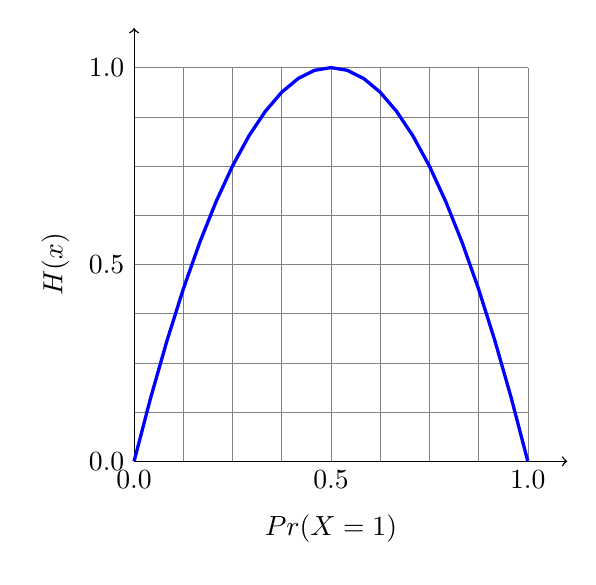
\begin{tikzpicture}[scale=5]
\draw[step=0.125, gray, very thin] (0,0) grid (1,1); 
\draw[->] (0,0) node[below]{0.0} -- (0.5,0) node[below]{0.5} (0.5,-.1)node[below,inner sep=5pt] {$Pr(X=1)$} (1,0)node[below]{1.0}--(1.1,0) ; 
\draw[->] (0,0) --(1.1,0);
\draw[->] (0,0) node[left]{0.0} -- (0,0.5) node[left]{0.5}
(-.2,0.5) node[align=left,inner sep=5pt, rotate=90] {$H(x)$} (0,1)node[left]{1.0}--(0,1.1) ; 
\draw[->] (0,0) --(0,1.1);
\draw[blue, very thick, domain=0:1] plot (\x, {4*\x-4*\x*\x}); 
\end{tikzpicture}
\end{document}
